\documentclass[mathserif,utf8,xcolor=table,10pt]{beamer}

\usepackage[T2A]{fontenc}
\usepackage[utf8]{inputenc}
\usepackage[english,russian]{babel}
\usepackage{graphicx}
\usepackage{ulem}
\usepackage{textpos}
\usepackage{hyperref}
%\usepackage{listings}
\usepackage{listingsutf8}
%\usepackage{minted}
\usepackage{tikz}
\usetikzlibrary{mindmap,shadows}
%\usepackage[hidelinks,pdfencoding=auto]{hyperref}


\definecolor{dkgreen}{rgb}{0,0.6,0}
\definecolor{gray}{rgb}{0.5,0.5,0.5}
\definecolor{mauve}{rgb}{0.58,0,0.82}

\lstset{frame=tb,
  language=C++,
%  aboveskip=3mm,
%  belowskip=3mm,
  showstringspaces=false,
  columns=flexible,
  basicstyle={\scriptsize\ttfamily},
  numbers=none,
  numberstyle=\tiny\color{gray},
  keywordstyle=\color{blue},
  commentstyle=\color{dkgreen},
  stringstyle=\color{mauve},
  breaklines=true,
%  breakatwhitespace=true,
  tabsize=2,
 % escapeinside={\%*}{*)},
 % inputencoding=utf8,
  inputencoding=utf8/utf8,
  texcl=true,
}

\mode<presentation>
{
        \usetheme{Antibes}
        \setbeamercovered{transparent}
}

\title{С++ продолжение. Организация совместной работы, системы контроля версий}
\institute{Степулёнок Денис Олегович}
\date[декабрь 2015]{23 декабря 2015 года}
\subject{Занятие 2}

\newcommand{\hl}{\only{\cellcolor{yellow}}}
\renewcommand{\le}{\leqslant}
\renewcommand{\ge}{\geqslant}
\setlength{\arrayrulewidth}{1pt}

\begin{document}

%\begin{frame}
%\titlepage
%\end{frame}

% Сложные типы данных в C/C++
% Массивы: одномерные, многомерные. 
% Записи (struct - структуры). typedef. Записи с вариантами (union). 

\section{Функции в C++}

\subsection{Рекурсия}
\begin{frame}[t,fragile]{Рекурсия - функция Факториал}
Итеративное вычисление факториала: от большего к меньшему $i = n, n-1, n-2 ... 2$
\begin{lstlisting}
long long factorial(int n) {
  long long r = 1; // Результат вычислений
  for(int i = n; i > 1; --i)
    r *= i; // Умножаем на i
  return r;
}
\end{lstlisting}

Цикл от меньшего к большему:
\begin{lstlisting}
  for(int i = 2; i <= n; ++i)
    r *= i;
\end{lstlisting}

\textbf{Рекурсия} --- когда функция вызывает сама себя.

Рекурсивный способ вычисления факториала:
\begin{lstlisting}
long long f(int n) {
  if(n <= 1)
    return 1; // Возвращаем 1
  else
    return n * f(n - 1); // Рекурсивный вызов
}
\end{lstlisting}

\end{frame}

\subsection{Передача параметров}

\begin{frame}[t,fragile]{Аргумент: значение, ссылка, указатель}
\begin{lstlisting}
// По значению - by value - копируется значение
// Внутри функции возникает новая переменная i, при изменении которой
// <<основная>> i никак не меняется
void f1(int  i) { i++;     cout << "i = " << i << endl;  }
// По ссылке - by reference - только в C++, но не в C
// i внутри функции - новое имя (алиас, alias) для внешней переменной
void f2(int& i) { i++;     cout << "i = " << i << endl;  }
// По указателю - by pointer
void f3(int* i) { (*i)++;  cout << "i = " << *i << endl; }

int main() { // Основная программа
  int i = 3; // <<Основная>> переменная i
    // Сначала она равна 3
  f1(i);  cout << "i = " << i << endl; // i = 3 по-прежнему
  f2(i);  cout << "i = " << i << endl; // i увеличилась
  f3(&i); cout << "i = " << i << endl; // i ещё раз увеличилась
  return 0;
}
\end{lstlisting}
\end{frame}

\begin{frame}[t,fragile]{Аргумент: по значению - <<обычная>> переменная}
\begin{lstlisting}
// По значению - by value - копируется значение
// Внутри функции возникает новая переменная i, при изменении которой
// "основная" i никак не меняется
void f1(int  i) { 
  i++;    
  cout << "i = " << i << endl; 
}
\end{lstlisting}

Внутри функции появляется новая переменная с тем значением, которое было передано внутрь функции.

Эту переменную можно использовать и менять как угодно и это никак не отразится на
переменной во внешней (вызывающей) программе.

Можно сказать, что эта переменная только для внутреннего использования.  

\end{frame}

\begin{frame}[t,fragile]{Аргумент: по ссылке - только в С++, не в C}
\begin{lstlisting}
// По ссылке - by reference
// i внутри функции - новое имя (алиас, alias) для внешней переменной
void f2(int& i) { 
  i++;     
  cout << "i = " << i << endl;  
}
\end{lstlisting}

Внутри функции появляется переменная, которая является другим именем для
внешней переменной.

Если мы поменяем значение переменной внутри функции, изменится и внешняя переменная.

Это можно использовать чтобы возвращать значения из функции. 
Или если функция должна менять значения в основной программе.
Например, есть какой-то глобальный счётчик и функция должна его увеличивать и ещё что-то.
\end{frame}

\begin{frame}[t,fragile]{Аргумент: по указателю}
\begin{lstlisting}
// По указателю - by pointer
void f3(int* i) { 
  (*i)++;  
  cout << "i = " << *i << endl; 
}
\end{lstlisting}

При этом внутри функции образуется новая переменная --- указатель на внешнюю переменную.

Сам указатель можно менять внутри функции.
Например, можно сделать чтобы он указывал на другую переменную.

Чтобы менять значение внешней переменной, нужно этот указатель
<<разыменовывать>>:

\begin{lstlisting}
  (*i) = 100;   
\end{lstlisting}

\end{frame}

\section{Ссылки и указатели в C++: общее и различия}

\begin{frame}[t,fragile]{C++ ссылка}
\textbf{Ссылка (reference)} --- это простой ссылочный тип, менее мощный, 
но более безопасный, чем указатель, унаследованный от языка C. 

С ссылкой нужно обращаться как с обычной переменной.
Например, её нельзя <<разыменовать>>.

Название <<C++ ссылка>> может приводить к путанице, 
так как в информатике под ссылкой понимается обобщенный концептуальный тип, 
а указатели и <<С++ ссылки>> являются специфическими реализациями ссылочного типа.
\end{frame}

\begin{frame}[t]{Отличия ссылки от указателя}
\begin{itemize}
\item Невозможно ссылаться напрямую на объект ссылочного типа после его определения; 
каждое упоминание его имени напрямую представляет объект, на который он ссылается.
\item При создании ссылки не могут быть выполнены никакие арифметические вычисления, приведения типов, взятия адреса и т.п.
\item После создания ссылки ее нельзя перевести на другой объект; в таких случаях говорят, не может быть \textbf{переопределена}. 
Это часто делают с указателями.
\item Ссылки не могут быть \texttt{NULL} (т.е. указывать в никуда), 
тогда как указатели - могут; 
каждая ссылка ссылается на некий объект, вне зависимости от его корректности.
\end{itemize}
\end{frame}

\begin{frame}[t,fragile]{Отличия ссылки от указателя...}
\begin{itemize}
\item Ссылки не могут быть неинициализированными. 
Так как невозможно переинициализировать ссылку, она должна быть инициализирована сразу после создания. 
В частности, локальные и глобальные переменные-ссылки должны быть проинициализированы там же, 
где они определены, а ссылки, которые являются данными-членами сущностей класса, 
должны быть инициализированы в списке инициализатора конструктора класса.
\end{itemize}
\begin{lstlisting}
 int& k; // компилятор выдаст сообщение: ошибка: 'k' declared as reference but not initialized 
         // ('k' объявлена как ссылка, но не инициализирована)
\end{lstlisting}
\end{frame}

\section{Структуры данных}

\begin{frame}[t,fragile]{Расстояние между 2-мя точками}

Точка на плоскости: задаётся 2-мя координатами: $(x; y)$

$dist(A, B) = \sqrt{{(A_x - B_x)^2} + {(A_y - B_y)^2}}$

\begin{lstlisting}
struct Point2D { double x, y; };

double dist(Point2D A, Point2D B) {
  return sqrt( pow(A.x - B.x, 2) + pow(A.y - B.y, 2));
}
\end{lstlisting}
\end{frame}

\begin{frame}[t,fragile]{Массивы}


\end{frame}



% 2. Организация совместной работы, системы контроля версий
% * Системы контроля версий: централизованные, распределённые
% * История версий, ветки
% * Основы работы с git
\section{Системы контроля версий}
\subsection{Что такое контроль версий, и зачем он вам нужен?}

\begin{frame}[t]{Что такое контроль версий, и зачем он вам нужен?}

Система контроля версий (СКВ) — это система, регистрирующая изменения в одном или нескольких файлах с тем, 
чтобы в дальнейшем была возможность вернуться к определённым старым версиям этих файлов. 

СКВ даёт возможность возвращать отдельные файлы к прежнему виду, 
возвращать к прежнему состоянию весь проект, 
просматривать происходящие со временем изменения, определять, 
кто последним вносил изменения во внезапно переставший работать модуль, 
кто и когда внёс в код какую-то ошибку, и многое другое. 
Вообще, если, пользуясь СКВ, вы всё испортите или потеряете файлы, всё можно будет легко восстановить. 

Системы контроля версий:
\begin{itemize}
  \item Централизованные 
  \item Децентрализованные
\end{itemize}

\end{frame}

\subsection{Системы контроля версий: локальные, централизованные, распределённые}

\begin{frame}[t]{Subversion}

Бесплатная система управления версиями с открытым исходным кодом.
Subversion позволяет управлять файлами и каталогами, а так же сделанными в них изменениями
во времени. Это позволяет восстановить более ранние версии данных, даѐт возможность изучить
историю всех изменений. Благодаря этому многие считают систему управления версиями своего
рода «машиной времени».

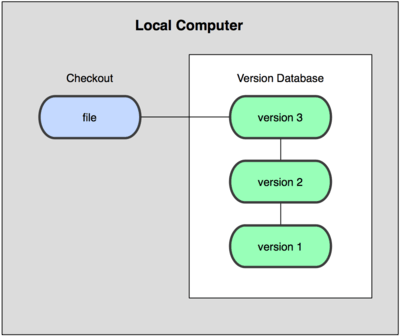
\includegraphics[width=0.5\textwidth]{git/rcs.png}

\end{frame}

\begin{frame}[t]{Централизованные системы контроля версий}
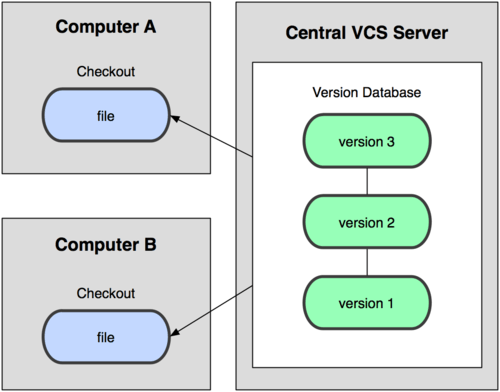
\includegraphics[width=0.5\textwidth]{git/central.png}
\end{frame}

\begin{frame}[t]{Распределённые системы контроля версий}
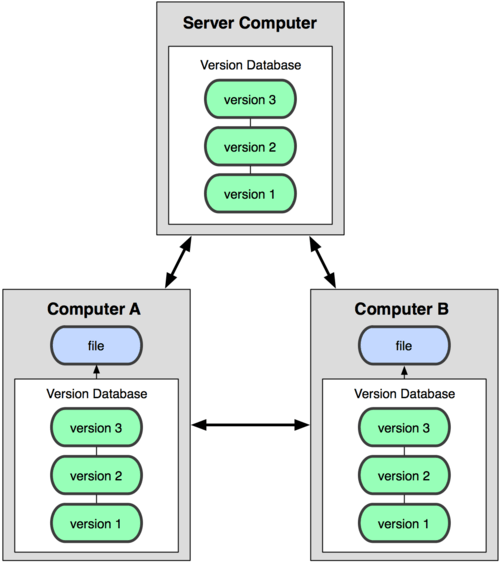
\includegraphics[width=0.5\textwidth]{git/distrib.png}
\end{frame}

\begin{frame}[t]{Git}

Распределённая система управления версиями. 
Проект был создан Линусом Торвальдсом для управления разработкой ядра Linux, первая версия выпущена 7 апреля 2005 года. 
На сегодняшний день его поддерживает Джунио Хамано.

Примерами проектов, использующих Git, являются:
ядро Linux, Android, Drupal, Cairo, GNU Core Utilities, Mesa, Wine, Chromium, Compiz Fusion, FlightGear, jQuery, PHP, NASM, MediaWiki, DokuWiki, Qt и некоторые дистрибутивы Linux 

\url{}

\end{frame}

\begin{frame}[t]{Откуда скачать и установить Git?}


Для Windows --- \url{https://git-for-windows.github.io}

Нажимаете \textbf{Download}, скачивается исполняемый файл, например 
\textbf{Git-2.6.1-64-bit.exe}

Устанавливаете его. 

После установки должна появится в командной строке команда:
\texttt{git}

\end{frame}

 
\subsection{История версий, ветки}
\begin{frame}[t]{Основные команды Git}

\texttt{git init} --- создание нового git-репозитория в текущей папке.
С этого момента в этой папке появляется <<машина времени>> для изменений.
Если вы сделали изменение и зафиксировали его, вы всегда можете откатиться к этой версии.

При успешной инициализации выводится сообщение:
Initialized empty Git repository in FolderName

\texttt{git add} --- добавление файлов в систему контроля версий.
Например: \texttt{git add a.cpp} --- добавить файл a.cpp в СКВ.
\texttt{git add *.cpp} --- добавить все .cpp файлы в СКВ. 
\texttt{git add .} --- добавить все файлы и все каталоги с подкаталогами в СКВ. 

\end{frame}

\subsection{Почитать про Git}
\begin{frame}[t]{Основные команды Git}

\end{frame}
                                         



% * Виды тестирования и отладки
\section{Тестирование и отладка}

\subsection{Методы тестирования и отладки}

\begin{frame}[t]{Методы тестирования и отладки}

  \begin{itemize}
    \item Ручное тестирование / ручная отладка --- Steps to reproduce / шаги "как воспроизвести" - 
      недостаток - слишком много ресурсов на повторение шагов каждый раз
    \item Использование отладчика (debugger)
    \item Логгирование (протоколирование) --- Единственный, который доступен на компьютере конечного пользователя
    \item Автоматические тесты
    \begin{itemize}
      \item Модульные: Unit-тесты
      \item Функциональные:
      \begin{itemize}
        \item По спецификации 
        \item Регрессионные тесты
      \end{itemize}
      \item Интеграционные тесты (integration)
      \item Тесты производительности (perfomance)
    \end{itemize}  
  \end{itemize}
\end{frame}


% Приоритет операций
\section{Приоритет операций в C/C++}

\subsection{Приоритет операций}

\begin{frame}[t,fragile]{Арифметические операции}

\begin{lstlisting}
  double x = 10 / 2 * 5;
  cout << "x = " << x << endl; // 25
  double x2 = 10 / (2 * 5);
  cout << "x2 = " << x2 << endl; // 1
  cout << 10.0 / 2.0 / 5.0 << endl; // 1.0
\end{lstlisting}

Всегда ставьте скобки, если не очевиден порядок.
 
\end{frame}


% * Модули: заголовочный файл (header), основной файл (.c и .cpp, .h и .hpp). 
\section{Типы данных С++}
\subsection{Целочисленные типы данных}

\begin{frame}[t]{Целочисленные типы данных}
  1 байт:
  \begin{itemize}
    \item \texttt{bool} --- логический тип данных: \texttt{true} / \texttt{false}
    \item \texttt{char} --- символьный тип данных от $-128$ до $127$ или $0..255$ \texttt{unsigned char}
  \end{itemize}
  2 байта:
  \begin{itemize}
    \item \texttt{short int}, \texttt{short} --- от $-2^{15}=-32.768$ до $2^{15}-1=32.767$
    \item \texttt{unsigned short int} --- от $0$ до $2^{16}-1=65.535$
  \end{itemize}
  4 байта:
  \begin{itemize}
    \item \texttt{int}, \texttt{long int}, \texttt{long}, \texttt{signed} --- от $-2^{31}=-2.147.483.648$ до $2^{31}-1=2.147.483.647$
    \item \texttt{unsigned int}, \texttt{unsigned long int}, \texttt{unsigned long}, \texttt{unsigned} --- от $0$ до $2^{32}-1=4.294.967.295$
  \end{itemize}
  8 байт:
  \begin{itemize}
    \item \texttt{long long, \_\_int64} --- от $-2^{63}=-9.223.372.036.854.775.808$ до $2^{63}-1=9.223.372.036.854.775.807$
    \item \texttt{unsigned long long, unsigned \_\_int64} --- от $0$ до $2^{64}-1=18.446.744.073.709.551.615$
  \end{itemize}
\end{frame}




% * Литература по C/C++.

\end{document}
